\chapter{Recreating winning approach}\label{sec:recreating}
This is the first chapter in the modelling part. In this chapter, the classification method of the Ford Competition winner will be attempted to be recreated. The goal is to get a result -- as measured by the AUC -- that is close to the winners approach.

\section{The winning approach}
The competition winner has described his approach in \citet{inference_winning_approach}, which will just be called ``the paper'' in the rest of this section. The main points in the paper will be described in this section. \par
In the paper two key observations are mentioned. First of all, the winner observed that in most of the trials, the driver was either alert most of the time, or not alert for most of the time. Secondly the winner observed that there was a mismatch between the AUC-scores achieved on the trainingset and on the testset. Since it wasn't possible to get access to the testset of the competition, the second observation isn't of any direct use for this report. The two observations though, gives an explanation of why the winner chose the model he did. \par
The fact that most trials was either alert-trials or not-alert-trials, the winner thought it would make sense to calculate aggregated features within trials. He therefore included the mean and the standard deviation of all features, aggregated backwards, within a trial. As a standard the mean features wasprefixed ``m'' and the standard deviation ``sd''. 
\begin{Exa}
    In the $k$'th observation of trial $t$, the value of feature \fn{mP6}, is the mean of feature \fn{P6}, for observation $0,1,2,\dots,k-1$ in trial $t$
\end{Exa}
The fact that there was a mismatch between the trainingset and testset of the competition, made the winner focus on simple models, since he expected that the trainingset wasn't capturing all aspects of the testset, and extrapolation was therefore needed.

\subsection{Classification method}
The method used by the winner was a logistic regression, trained on only the three features \fn{sdE5}, \fn{V11} and \fn{E9}. The three features was selected ``... based on diagnostics of the logistic regression ...'' \citep[p.3]{inference_winning_approach}. The final model was a logistic regression with the following weights
\[
    \log\frac{P(t=0|\ve{x})}{P(t=1|\ve{x})} = -392.4317\cdot\text{sdE5} + 0.2209\cdot\text{V11} + 3.6544\cdot\text{E9}
\]
\begin{figure}\label{fig:auc-score-inference-paper}
    \centering
    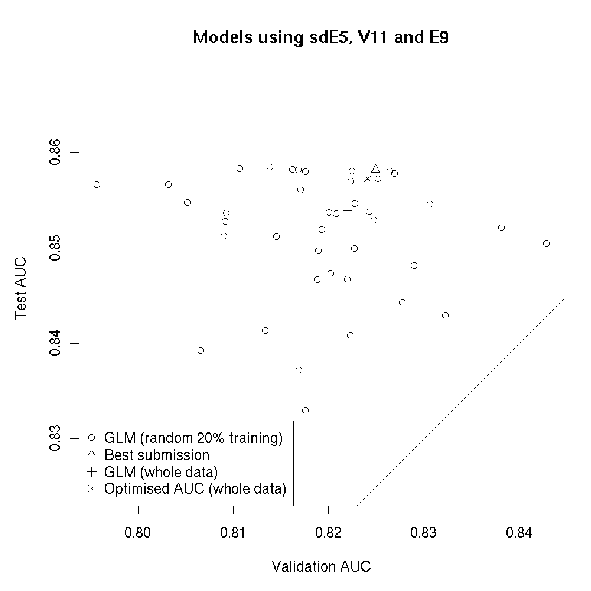
\includegraphics[width=100mm]{media/fig2-inference-paper.pdf}
    \caption{Reproduction of figure 2 in \citet{inference_winning_approach}. The models that achieves a Test AUC higher than 0.8492 are using future observations to predict the \fn{IsAlert} feature, which wasn't allowed in the competition. See \citet{inference_winning_approach} for more information.}
\end{figure}
The winner do not mention any intercept parameter, although it seems unlikely that no intercept was included in the model \citep{meetings-morten}. Based on the above parameters, the winner achieved an AUC-score of 0.8492 on the testset. As mentioned in the previous section, the AUC-score of the testset differed from the AUC-score on the trainingset. In figure 2 in \citet{inference_winning_approach}  it is seen that an AUC-score of 0.8492 on the testset, corresponded to a AUC-score of $0.82\pm0.01$ on the trainingset. Since only the trainingset is available for this report, the goal is to acieve an AUC-score of approximately $0.82\pm0.01$.

\section{Recreating the winning approach}
It is now time to recreate the logistic regression of the winner. A 10-fold cross validation method is used. The trainingset is therefore split in 10 parts, and one part is repeatedly used as validationset while the other 9 parts, are used to train the logistic regression. This gives 10 estimates of the true AUC-score, and 10 different parameter vectors. The results can be seen in table~\ref{tbl:recreate-results} and the source code used to calculate the results can be found in \appref{source-recreate-winner} \par
\begin{table}
    {\sffamily\small
    \begin{tabularx}{\textwidth}{ l R R R R R }
        Run & sdE5 & V11 & E9 & Intercept & AUC \\\hline
        1 & -87.2063 & 0.2239 & 3.6578 & -5.3642 & 0.8051 \\
        2 & -353.2778 & 0.2157 & 3.6969 & -4.9869 & 0.8185 \\
        3 & -87.4096 & 0.2246 & 3.6644 & -5.3763 & 0.8048 \\
        4 & -352.1050 & 0.2159 & 3.6960 & -4.9905 & 0.8208 \\
        5 & -86.9788 & 0.2231 & 3.6455 & -5.3440 & 0.8097 \\
        6 & -87.1768 & 0.2239 & 3.6487 & -5.3539 & 0.8060 \\
        7 & -87.1603 & 0.2244 & 3.6575 & -5.3666 & 0.8074 \\
        8 & -87.3095 & 0.2245 & 3.6618 & -5.3736 & 0.8078 \\
        9 & -353.1568 & 0.2150 & 3.6951 & -4.9778 & 0.8177 \\
        10 & -87.3047 & 0.2245 & 3.6461 & -5.3590 & 0.8095 \\\hline
    \end{tabularx}
    }
    \caption{Results of running a 10-fold cross validation logistic regression, on the features used by the winner.}
    \label{tbl:recreate-results}
\end{table}
From the results table it is seen that the single best run is the fourth run, that gives the model
\[
    \log\frac{P(t=0|\ve{x})}{P(t=1|\ve{x})} = -352.1050\cdot\text{sdE5} + 0.2159\cdot\text{V11} + 3.6960\cdot\text{E9} - 4.9905
\]
This model achieves an AUC-score of 0.8208 on the validationset. From the results, it is also seen that there are two distinct patterns in the parameters, that are given by the logistic regression. On 7 out of the 10 runs the weight of the \fn{sdE5} feature is about 87 and on the rest of the runs it is 352-353. The runs with a \fn{sdE5}  weight around 352-353 are consistently giving better AUC-scores than the other runs. The three runs with the \fn{sdE5} feature of 352-353, all have feature weights that is close to the weights used in the winning model. The AUC-scores achieved by theese three models also comes close to the AUC-scores of the winner.

\subsection{Statistics on the AUC score}
From the results of the 10-fold cross validation logistic regression, 10 AUC scores was obtained. If it is assumed that the 10 AUC scores are a sample from the population of all AUC scores on unknown datasets, a confidence interval for the AUC score can be calculated. The mean $\widehat{\mu}$ and standard deviation $\widehat{\sigma}$ of the AUC score are calculated as
\[
\widehat{\mu} = 0.8107 \quad\quad\text{and}\quad\quad \widehat{\sigma} = 0.005980
\]
\mytodo{Calculate confidence interval for AUC estimate}
